\documentclass[12pt]{article}

\usepackage{preamble}

%title, author, date
\title{Netzwerkanalyse mit Wireshark: Was passiert im Netzwerk?}
\author{Luis Herzog}


\begin{document}

%Titlepage

\maketitle

\begin{figure}[h]
	\centering
	
\includegraphics[scale=0.1]{Bilder/Wireshark_icon.svg.png}
	\caption{Wireshark Logo \cite{wireshark-logo}}
	\label{fig:figure1}
\end{figure}

\thispagestyle{empty}
\newpage
\tableofcontents
\thispagestyle{empty}
\newpage

\section{Vorwort}
Die Digitalisierung ist in aller Munde. Durch die Digitalisierung wächst die Anzahl von Netzwerken, nicht nur in Deutschland, sondern weltweit. Netzwerke werden überall benutzt. Die meisten Menschen besitzen Heimnetzwerke. Aber es gibt noch viel mehr Netzwerke, zum Beispiel in Flughäfen, Cafés, Bibliotheken und noch so viel mehr. Diese Vielfalt von Netzwerken lässt einen Gedanken aufleuchten: \glqq Wie funktionieren Netzwerke?\grqq. 
Durch die Digitalisierung haben sich Netzwerke stark verändert und vor allem vergrößert. Dadurch sind Netzwerke oft sehr komplex. Die Wireshark Software erlaubt es, einen tieferen Blick in das Netzwerk zu werfen und Details herauszufinden. In dieser Arbeit wird die Arbeitsweise eines Netzwerks dargelegt und die Wireshark Software erklärt. 


Bevor man über die Wireshark Software sprechen kann, müssen die fundamentalen Fakten geklärt werden:

\section{Daten}
Statista, eine Website für Statistiken,  beschreibt Daten als \glqq Messwerte, die im Rahmen von Befragungen, Beobachtungen oder Experimenten erhoben werden\grqq. \cite{statista-daten} Der Duden gibt mehrere Definitionen. Die dritte Definition gibt Daten als \glqq elektronisch gespeicherte Zeichen, Angaben, Informationen\grqq\cite{duden-daten} an. Da es viele verschiedene Arten von Daten gibt, gibt es viele verschiedene Definitionen. Im Netzwerk beschreiben Daten den Inhalt und Aufbau von Paketen. Zum Inhalt gehören Informationen zum Paket und die zu vermittelnde Nachricht, welche alle durch elektronisch gespeicherte Zeichen dargestellt werden.

\subsection{Metadaten}
Metadaten spielen hierbei ebenfalls eine wichtige Rolle. Diese Daten sind die schon oben genannten Informationen über weitere Daten. Mit diesen Metadaten lässt sich ein zugehöriger Inhalt besser Einordnen, Katalogisieren und Analysieren. Metadaten sind strukturierte Daten und können bei physischen Gegenständen sowie bei digitalen Dateien Einsatz finden. Ein Beispiel für Metadaten ist der Autor bei einem Buch oder der Komponist bei einem Musikstück.\cite{metadaten-security-insider} In der Netzwerktechnik sind Metadaten besonders wichtig. Diese sind im Adresskopf der Datenpakete gespeichert und enthalten beispielsweise Informationen über die Quelladresse und Zieladresse des Pakets, sowie über die Lebensdauer des Pakets.\cite{tcp+ip-netzwerkecom} Mehr hierzu wird später im Kapitel 4 unter \glq Exkurs: UDP/TCP\grq erklärt.

\section{Das Programm: Wireshark}

Heise.de bezeichnet Wireshark als \glqq Schweizer Taschenmesser\grqq\cite{schweizer-taschenmesser} der Netzwerktechnik. Das Programm wird fast überall in der IT-Branche benutzt. Sei es beim Finden von Netzwerkproblemen oder beim Lernen, wie ein Netzwerk funktioniert. Somit bietet das Programm eine Menge Möglichkeiten. Wireshark ist ein \glqq network packet analyzer\grqq\cite{what-is-wireshark}. Es erlaubt dem Benutzer den Netzwerkverkehr aufzunehmen und zu analysieren. Mit Wireshark kann man sozusagen in ein Netzwerkkabel \glq hineinschauen\grq.

\subsection{Geschichte}
Wireshark wurde 1997 von Gerald Combs als \glq Ethereal\grq ins Leben gerufen. Das Programm wurde im Juli 1998 als Version 0.2.0 unter einer GPL Lizenz\cite{gnu-gpl} herausgegeben \cite{gnu-wireshark} Somit konnten viele Menschen am Code des Programms mithelfen, um es zu verbessern. Im Jahr 2006 wurde das Projekt in \glq Wireshark\grq umbenannt. Anschließend wurde  im Jahr 2008 die Version 1.0 als erste komplette Version veröffentlicht. Sieben Jahre später wurde 2015 die Version 2.0 mit einem komplett neuen Benutzeroberfläche vorgestellt. Letztendlich wurde im Jahr 2023 die Wireshark Foundation\footnote{https://wiresharkfoundation.org/} gegründet, welche jetzt das Programm unterstützt. \cite{wireshark-history}

\subsection{Funktionsumfang}

Wireshark bietet fast alles rund um das Thema Netzwerkanalyse. Mit Wireshark kann man den Netzwerkverkehr aufnehmen, mit hohem Detail darstellen und einfach exportieren oder speichern. Außerdem kann man diese exportierten Netzwerkdumps von Wireshark und anderen Programmen wieder importieren. Da Wireshark sowohl auf UNIX Platformen als auch auf Windows verfügbar ist, geht dies Plattformübergreifend. Ebenso kann man die Datenpakete anhand verschiedener Kriterien filtern und durchsuchen. Die genannten Funktionen kratzen aber nur an der Oberfläche. Wireshark bietet noch viel mehr Funktionen.\cite{features}

\subsection{Benutzeroberfläche}

Das voreingestellte Layout ist im folgenden Screenshot (siehe Abbildung 2) dargestellt. In diesem Fall wird gerade die Netzwerkschnittstelle `wg-mullvad` aufgezeichnet. Im oberen Teil ist die Symbolleiste zu sehen. Dort findet man Knöpfe zum Starten und Stoppen der Aufnahme.  Rechts daneben befinden sich die Knöpfe zum Laden und Speichern von Netzwerkdumps. Weiter rechts folgen Knöpfe zum Sortieren der Paketliste. Darunter befindet sich die Liste mit den aufgenommenen Paketen. Dort kann direkt die Zeit, die Quelle und das Ziel des Pakets abgelesen werden. Rechts daneben ist das genutzte Netzwerkprotokoll und die Länge des Pakets sichtbar. Ganz rechts stehen weitere Information zum Paket. Unter dieser Liste befinden sich zwei Fenster. Rechts steht die Rohdaten des Pakets. Links hingegen steht der von Wireshark automatisch ausgelesene und geordnete Inhalt. Hier kann jegliche Information zum Datenpaket gefunden werden. Unter diesem Fenster steht der Name der Netzwerkschnittstelle, deren Netzwerkverkehr aufgezeichnet wird.


\begin{figure}[h]
	\begin{center}
		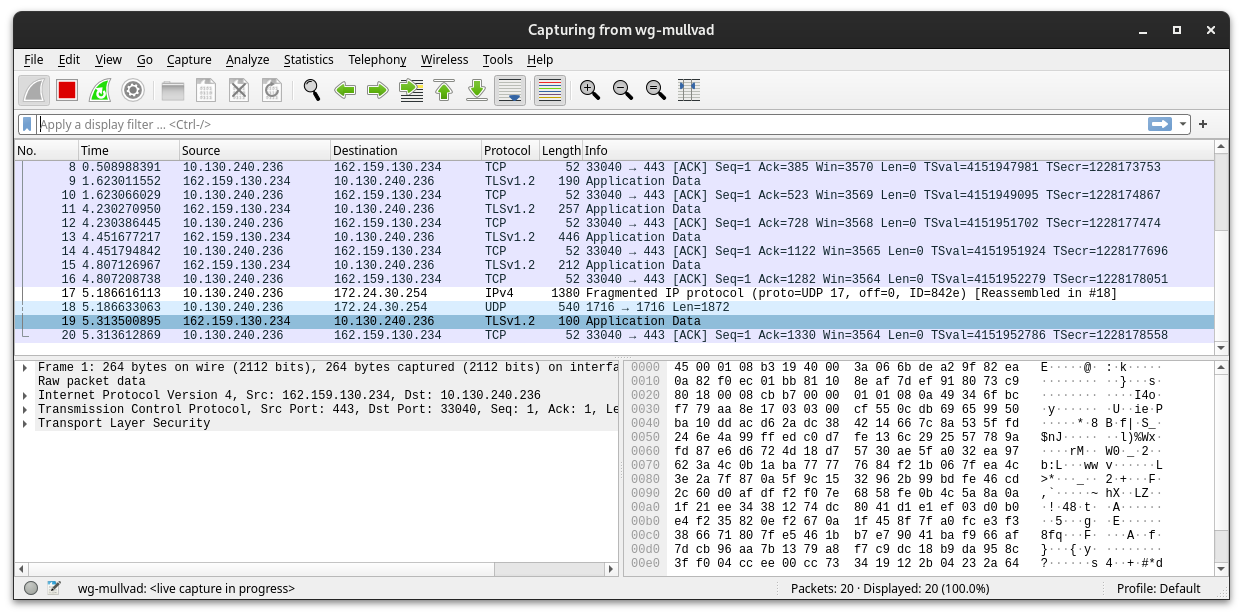
\includegraphics[scale=0.25]{Bilder/Screenshot_1.png}
		\label{fig:figure2}
		\caption{Beispielscreenshot aus der Wireshark Software \cite{screenshots-self}}
	\end{center}
\end{figure}



\subsection{Anwendungsbereiche}
Wie schon im oberen Teil dargestellt, bietet Wireshark sehr viele Funktionen. Es kann in sehr vielen Situationen Anwendung finden. Es wird beispielsweise von Netzwerk Administratoren zum Finden, Analysieren und Lösen von Netzwerkproblemen benutzt. Das Programm kann auch von Sicherheitsanalysten benutzt werden, um Sicherheitsprobleme in Netzwerken zu finden. Von Anwendungsentwicklern wird Wireshark benutzt, um die Umsetzung von Netzwerkprotokollen auszutesten. Eine weitere Anwendung ergibt sich beim Lernen, über das Netzwerk durch Wireshark. Es gibt natürlich auch viele weitere Möglichkeiten das Programm zu benutzen.\cite{intended-purposes}

\section{Netzwerk}
In der Informationstechnologie ist ein Netzwerk ein Zusammenschluss mehrerer Computer [...], die untereinander kommunizieren, also Daten untereinander austauschen können.\cite{netzwerk-kurthelec}
\subsection{Aufbau}

\begin{wrapfigure}{r}{0.65\textwidth}
	\centering
	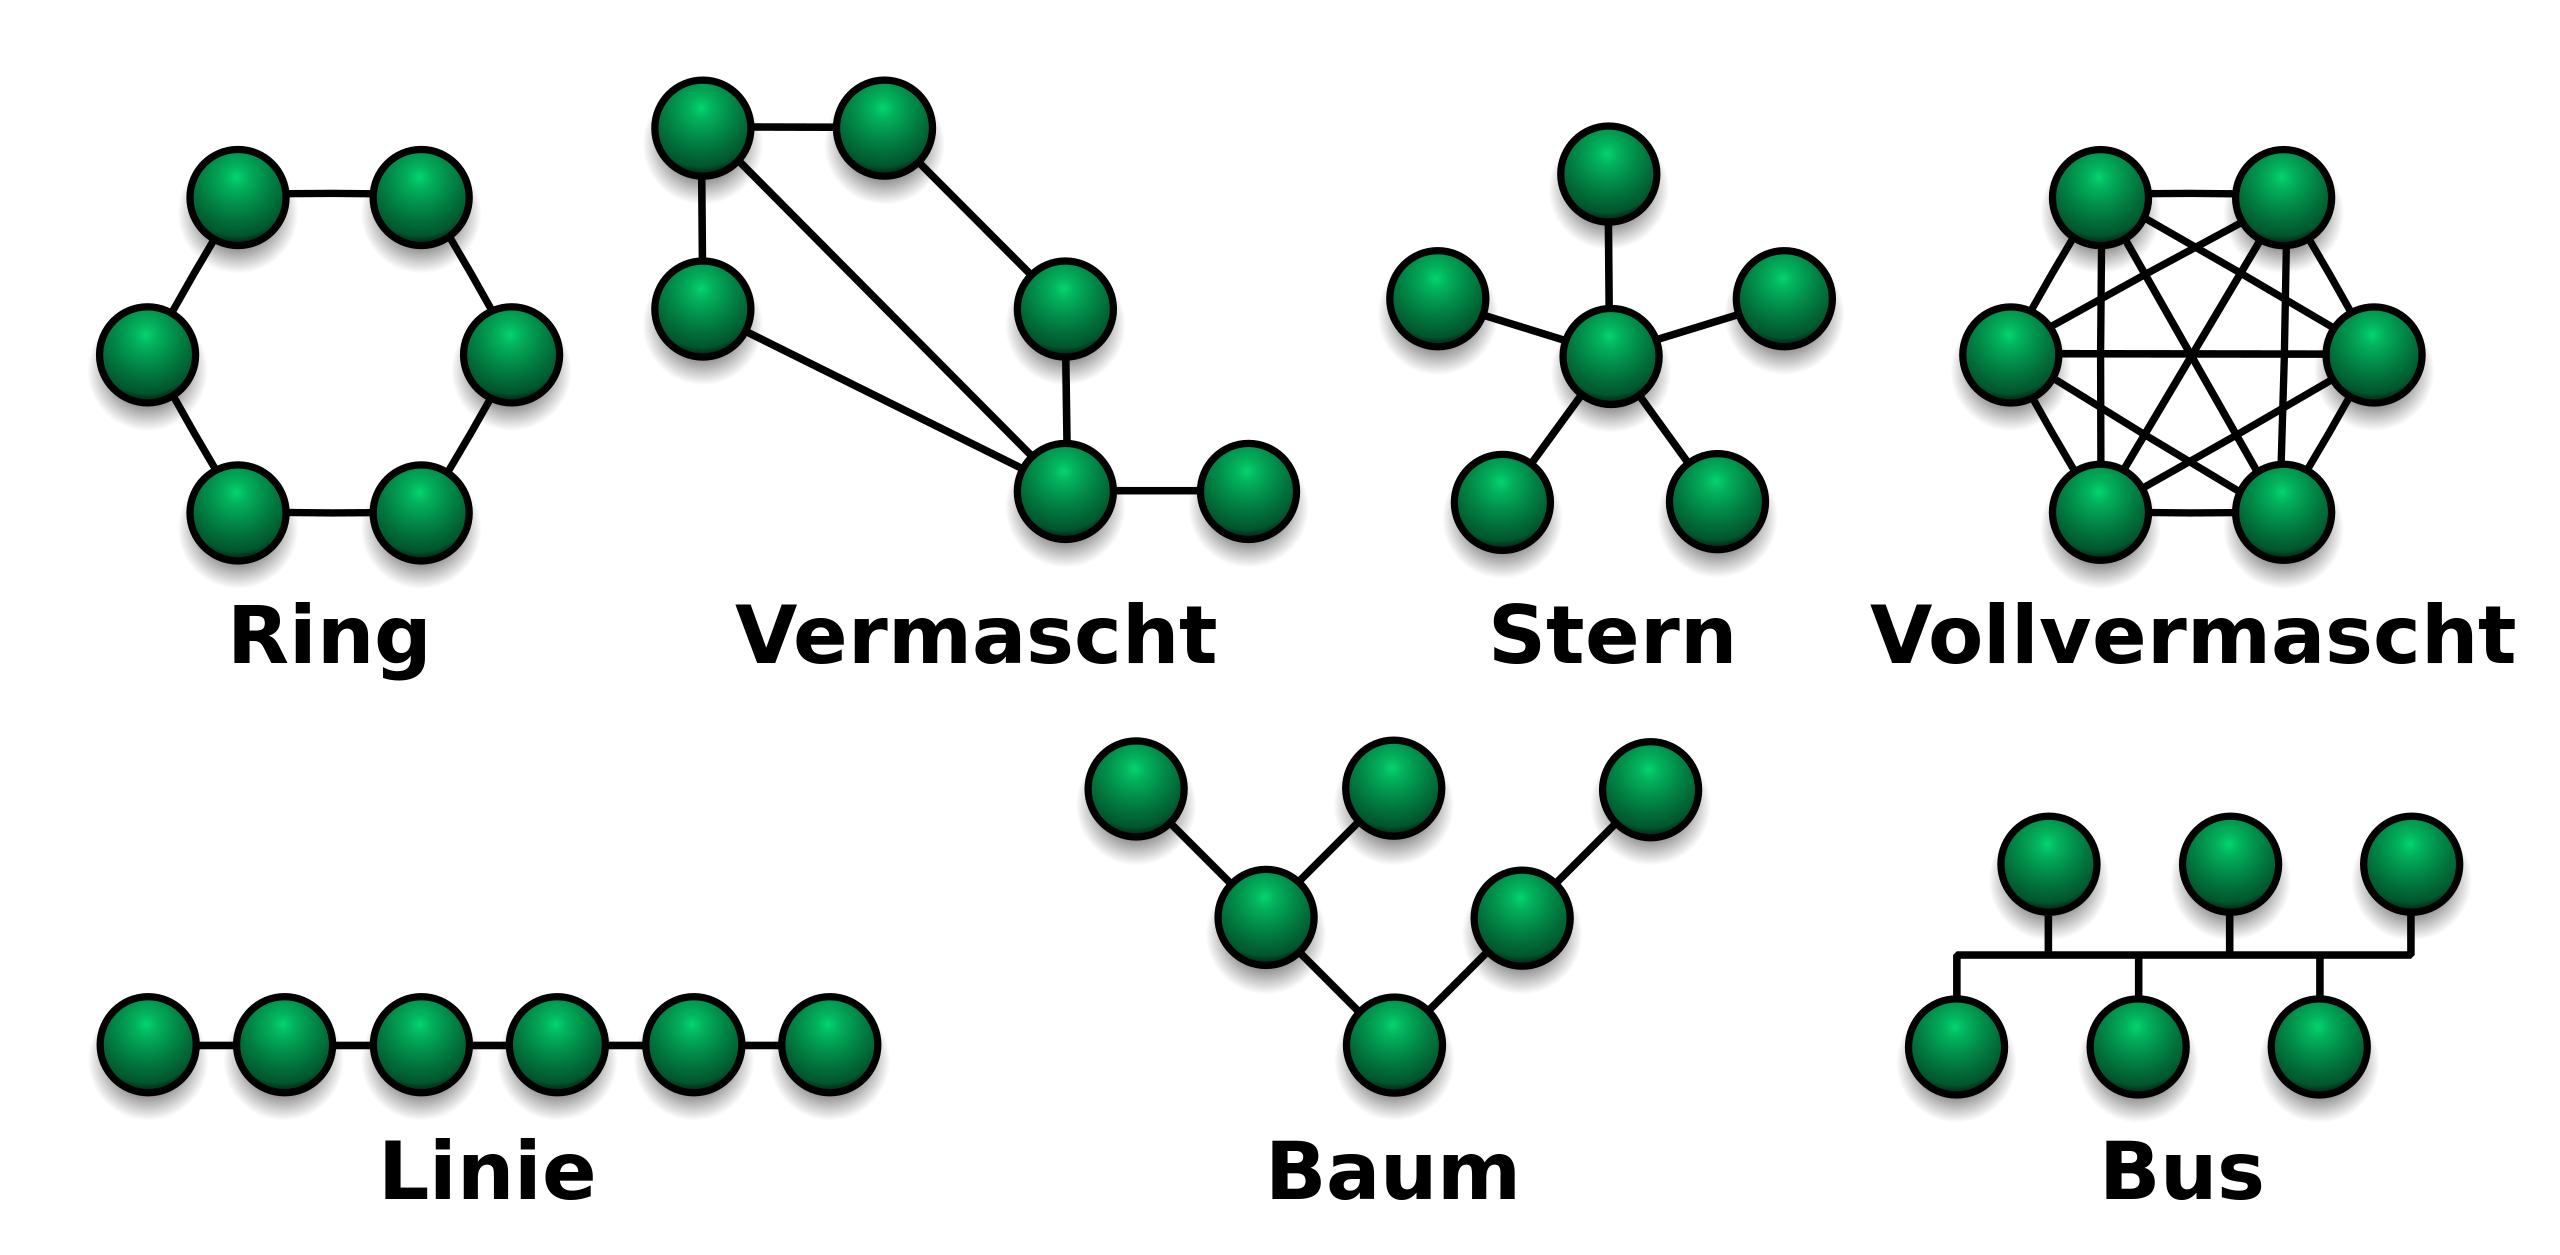
\includegraphics[scale=0.1]{Bilder/NetzwerkTopologien.svg}
	\caption{Die Netzwerktopologien \cite{topologien-darstellung}}
	\label{fig:figure5}
\end{wrapfigure}

Es gibt viele verschiedene Arten von Netzwerken, die unterschiedlich aufgebaut  sein können. Netzwerke werden in Topologien unterteilt. Durch diese Topologien können selbst sehr komplexe Netzwerke gut veranschaulicht werden. Es gibt fünf Haupttopologien. Bei der Ringtopologie sind alle Knoten in einem Ring miteinander verbunden. Die Linientopologie ist ähnlich, mit dem Unterschied, dass die Knoten an den Enden nicht mehr direkt miteinander verbunden sind. Bei der Sterntopologie sind alle Knoten mit einem Hauptknoten verbunden. Die Baumtopologie ist eine erweiterte Form der Sterntopologie, bei der mehrere Knoten hierarchisch miteinander verbunden sind. Bei der Bustopologie hängen alle Knoten an einem Übertragungsmedium. Netzwerke können ebenfalls vermascht sein, was bedeutet, dass die Knoten mehr Verbindungen aufweisen, als theoretisch nötig wären. Bei einem vollvermaschten Netzwerk ist jeder Knoten mit allen weiteren Knoten verbunden.\cite{topologien-kurthelec} Der Beispielaufbau in Abbildung 4 zeigt ein Netzwerk basierend auf der Sterntopologie.

\begin{figure}[h]
	\centering
	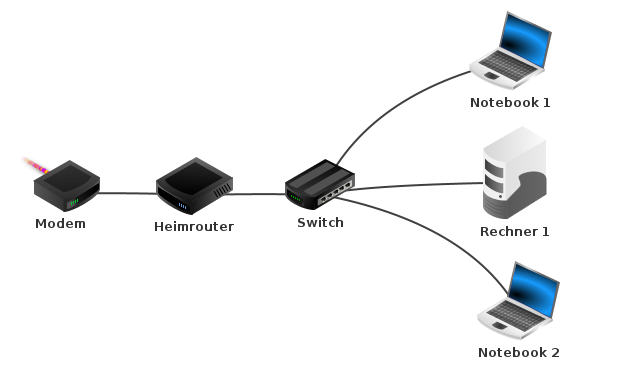
\includegraphics[scale=0.7]{Bilder/beispielnetzwerk}
	\caption{Aufbau eines Beispielnetzwerks \cite{network-self}}
	\label{fig:figure4}
\end{figure}






\subsection{Protokolle}

Damit alle Komponenten im Netzwerk richtig miteinander kommunizieren können, wurden standardisierte Protokolle entwickelt. Somit  sprechen alle Komponenten \glq die gleiche Sprache\grq. Es gibt verschiedene Protokolle für verschiedene Zwecke. Beispielsweise gibt es HTTP für den Transfer von Websiten oder FTP zum Senden von Dateien. Da es sehr viele Protokolle gibt und diese recht komplex aufgebaut sind, gibt es das OSI-Modell, um den Netzwerkverkehr mit Protokollen vereinfacht darzustellen. Im nächsten Abschnitt wird dieses Modell genauer beleuchtet.

\newpage
\subsection{Open System Interconnection Model}


	
	\begin{wraptable}{r}{0pt}
		\centering
		\resizebox{0.6\textwidth}{!}{
			\begin{tabular}{|
					>{\columncolor[HTML]{C0C0C0}}l 
					>{\columncolor[HTML]{9B9B9B}}l l|}
				\hline
				\multicolumn{3}{|l|}{\cellcolor[HTML]{FFFFFF}OSI-Modell}                                                                                                             \\ \hline
				\multicolumn{1}{|l|}{\cellcolor[HTML]{C0C0C0}}                               & \multicolumn{1}{l|}{\cellcolor[HTML]{9B9B9B}7} & \cellcolor[HTML]{34FF34}Application  \\ \cline{2-3} 
				\multicolumn{1}{|l|}{\cellcolor[HTML]{C0C0C0}}                               & \multicolumn{1}{l|}{\cellcolor[HTML]{9B9B9B}6} & \cellcolor[HTML]{34FF34}Presentation \\ \cline{2-3} 
				\multicolumn{1}{|l|}{\cellcolor[HTML]{C0C0C0}}                               & \multicolumn{1}{l|}{\cellcolor[HTML]{9B9B9B}5} & \cellcolor[HTML]{34FF34}Session      \\ \cline{2-3} 
				\multicolumn{1}{|l|}{\multirow{-4}{*}{\cellcolor[HTML]{C0C0C0}Host Layers}}  & \multicolumn{1}{l|}{\cellcolor[HTML]{9B9B9B}4} & \cellcolor[HTML]{67FD9A}Transport    \\ \hline
				\multicolumn{1}{|l|}{\cellcolor[HTML]{C0C0C0}}                               & \multicolumn{1}{l|}{\cellcolor[HTML]{9B9B9B}3} & \cellcolor[HTML]{F8FF00}Network      \\ \cline{2-3} 
				\multicolumn{1}{|l|}{\cellcolor[HTML]{C0C0C0}}                               & \multicolumn{1}{l|}{\cellcolor[HTML]{9B9B9B}2} & \cellcolor[HTML]{F56B00}Data Link    \\ \cline{2-3} 
				\multicolumn{1}{|l|}{\multirow{-3}{*}{\cellcolor[HTML]{C0C0C0}Media Layers}} & \multicolumn{1}{l|}{\cellcolor[HTML]{9B9B9B}1} & \cellcolor[HTML]{FE0000}Physical     \\ \hline
			\end{tabular}%
		}
			\caption{OSI-Modell \cite{osi-table}}
		\label{fig:figure3}
	\end{wraptable}

	


	Das Open System Interconnect\footnote{dt: Offenes System für Kommunikationsverbindungen} Modell, auch OSI-Modell genannt, beschreibt die Voraussetzungen, die für eine Kommunikation innerhalb eines Netzwerks nötig sind. Dieses wurde 1983 von der \glq Internationalen Organisation für Normung\grq standardisiert. Diese Standardisierung ist notwendig, damit sich alle Komponenten im Netzwerk, auch wenn diese von verschiedenen Herstellern produziert wurden, reibungslos miteinander funktionieren. Wenn ein Paket beispielsweise von einem Computer im Netzwerk losgeschickt wird, muss es mehrere Stationen durchlaufen. Das Paket verlässt den Rechner über die Netzwerkkarte und wird durch ein Übertragungsmedium über weitere Netzwerkkomponenten wie Hubs oder Router bis zur Netzwerkkarte des Zielrechners geleitet. Dort wird dieses Interpretiert, um korrekt dargestellt zu werden. All diese Schritte werden durch ein Protokoll festgehalten und durch das OSI-Modell spezifiziert, damit jede Station auf diesem Weg weiß, wohin das Paket möchte, woher es kommt und welche Eigenschaften es hat. So wird ein Standard geschaffen, mit dem alle Computersysteme arbeiten können.
	
	Da diese  Datenkommunikation relativ komplex ist, wurde das Modell in sieben Schichten eingeteilt. Die oberen vier Schichten gehören zu den anwendungsorientierten Schichten\footnote{engl: host layer}. Die unteren drei Schichten werden Transportschichten\footnote{engl: media layer} genannt. Jede Schicht behandelt eine Anforderung, die für eine funktionierende Kommunikation erfüllt werden muss. Ein zu übertragendes Paket durchläuft vor der Versendung die Schichten 7 - 2, wobei dem Paket bei jeder Schicht Protokollinformationen hinzugefügt werden, die dann im Protokoll des Datenpaketes auffindbar sind. Die erste und letzte Schicht wandelt das Paket in technisch übertragbare Daten um und schickt dieses über das Übertragungsmedium weg. Das Medium kann hierbei ein Kabel sein oder aus einer Antenne bestehen. Auf der Empfängerseite wird dieser Prozess rückwärts durchgeführt. Hierbei wird die jeweilige Protokollinformation nach der Interpretierung durch die zuständige Schicht entfernt, bis der Inhalt des Pakets zum Vorschein kommt.\cite{osi-netzwerkecom}
	
	Im Folgenden werden die einzelnen Schichten beleuchtet, um einen besseren Einblick in die Datenübertragung zu gewähren.

\subsubsection{Anwendungsschicht}
	Die Anwendungsschicht\footnote{engl: application layer} stellt die Daten dar, mit welchen der Nutzer interagiert. Softwareanwendungen, wie Webbrowser und E-Mail-Clients stützen sich auf die siebte Schicht, um dem Nutzer aussagekräftige Daten zu präsentieren. 
	
	Hierzu gehören Protokolle, wie HTTP\footnote{Hyper Text Transfer Protocol}, welches benutzt wird, um Websites welche in HTML\footnote{Hyper Text Markup Language} geschrieben sind zu präsentieren, oder SMTP\footnote{Simple Mail Transfer Protocol}, welches benutzt wird um E-Mails darzustellen.\cite{osi-schichten-cloudflare}\cite{osi-schichten-netzwerkecom}

\subsubsection{Präsentationsschicht}
	Die Präsentationsschicht\footnote{engl: presentation layer} ist in erster Linie dafür verantwortlich, die Daten so aufzubereiten, dass diese in der Anwendungsschicht verwendet werden können. Ein wichtiger Teil dabei ist die Verschlüsselung. Die Präsentationsschicht muss, wenn die Geräte durch eine verschlüsselte Verbindung kommunizieren, auf Senderseite eine Verschlüsselung hinzufügen und diese auf der Empfängerseite korrekt dekodieren. 
	
	Ebenso ist die Präsentationsschicht für die Komprimierung der Daten verantwortlich. Dadurch kann die Geschwindigkeit und Effizienz der Kommunikation erhöht und die benötigte Bandbreite minimiert werden.\cite{osi-schichten-cloudflare}\cite{osi-schichten-netzwerkecom}

\subsubsection{Sitzungsschicht}
	Anschließend folgt die Sitzungsschicht\footnote{engl: session layer}. Diese ist für das Öffnen und Schließen der Kommunikation der beiden Geräte zuständig. Hier wird die Kommunikation in Sitzungen eingeteilt. Eine Sitzung reicht von der Öffnung bis zur Schließung der Verbindung. Somit wird sicher gestellt, dass die Sitzung lange genug geöffnet bleibt, um alle Daten zu übertragen. Wenn alle Daten erfolgreich übertragen wurden, leitet die Sitzungsschicht die umgehende Schließung der Sitzung ein, um Ressourcen zu sparen. 
	
	Eine weitere sehr wichtige Aufgabe der Sitzungsschicht ist die Sicherung der Datenverbindung durch synchronisierte Checkpoints. Wenn beispielsweise bei der Übertragung einer 450 Megabyte großen Datei bei 234 Megabyte die Verbindung unterbrochen wird, kann nach einer Neuverbindung die Übertragung bei z.B. 230 Megabyte wieder aufgenommen werden, da es einen Checkpoint der Datei bei 230 Megabyte gibt.\cite{osi-schichten-cloudflare}\cite{osi-schichten-netzwerkecom}

\subsubsection{Transportschicht}
	In der Transportschicht\footnote{engl: transport layer} werden die Datenpakete vor dem Versenden in Segmente zerlegt. Im Empfangsgerät werden diese Segmente durch die Transportschicht wieder korrekt zusammengesetzt, sodass diese von der Sitzungsschicht benutzt werden können. 
	
	Die Transportebene ist ebenfalls für die Fluss- und Fehlersteuerung zuständig. Hierbei wird die Übertragungsgeschwindigkeit so festgelegt, dass ein ggf. langsamer Empfänger nicht durch die ggf. schnelle Geschwindigkeit des Senders überfordert wird. Beim Empfänger wird durch die Fehlersteuerung ein vollständiger Empfang aller Daten sichergestellt. Wenn die empfangenen Daten nicht vollständig sind, werden diese durch dieses System erneut angefordert, um die Vollständigkeit der Daten zu garantieren. 
	
	Hierzu gehören die Protokolle TCP\footnote{Transmission Control Protocol} und UDP\footnote{User Datagram Protocol}\cite{osi-schichten-cloudflare}\cite{osi-schichten-netzwerkecom}

\subsubsection{Exkurs: UDP/TCP}

Die zwei Protokolle UDP und TCP sind die meist verwendeten Protokolle, weswegen die Protokolle in den oberen Schichten darauf aufbauen. 

TCP ist ein verbindungsorientertes Protokoll. Der Client und der Server müssen erst eine Verbindung herstellen, damit Daten in beide Richtungen übertragen werden können. TCP verfügt außerdem über ein erhebliches System für die Fehlerkontrolle durch beispielsweise Prüfsummen.\cite{tcp+ip-netzwerkecom} Dadurch ist TCP ein sehr zuverlässiges, aber eher langsames Protokoll. Es wird benutzt, um Dateien, Websites oder Bilder zu übertragen.\cite{tcp} In Tabelle 2 sind die Eigenschaften übersichtlich aufgefächert.

\begin{table}[h]
	\resizebox{\textwidth}{!}{%
		\begin{tabular}{|
				>{\columncolor[HTML]{C0C0C0}}l |
				>{\columncolor[HTML]{8feb34}}l |}
			\hline
			\cellcolor[HTML]{9B9B9B}Eigentschaften                        & \cellcolor[HTML]{9B9B9B}TCP                               \\ \hline
			Verbindungsstatus                     & Erfordert eine bestehende Verbindung zur Datenübertragung \\ \hline
			Datensequenzierung                    & Erfordert Sequenzierung                                   \\ \hline
			Garantierte Übertragung               & Übertragung wird garantiert                               \\ \hline
			Neuübertragung von verlorenen Paketen & Neuübertragung von verlorenen Paketen ist möglich         \\ \hline
			Fehlerüberprüfung                     & Umfangreiche Fehlerüberpfüfung und Bestätigen der Daten   \\ \hline
			Geschwindigkeit                       & Langsamer als  UDP                                        \\ \hline
			bestmögliche Verwendung               & Streaming bei Videokonferenzen, VoIP oder Livestreams     \\ \hline
		\end{tabular}%
	}
	\caption{TCP \cite{udp+tcp}}
	\label{fig:figure11}
\end{table}



\begin{wrapfigure}{r}{0.5\textwidth}
	\centering
	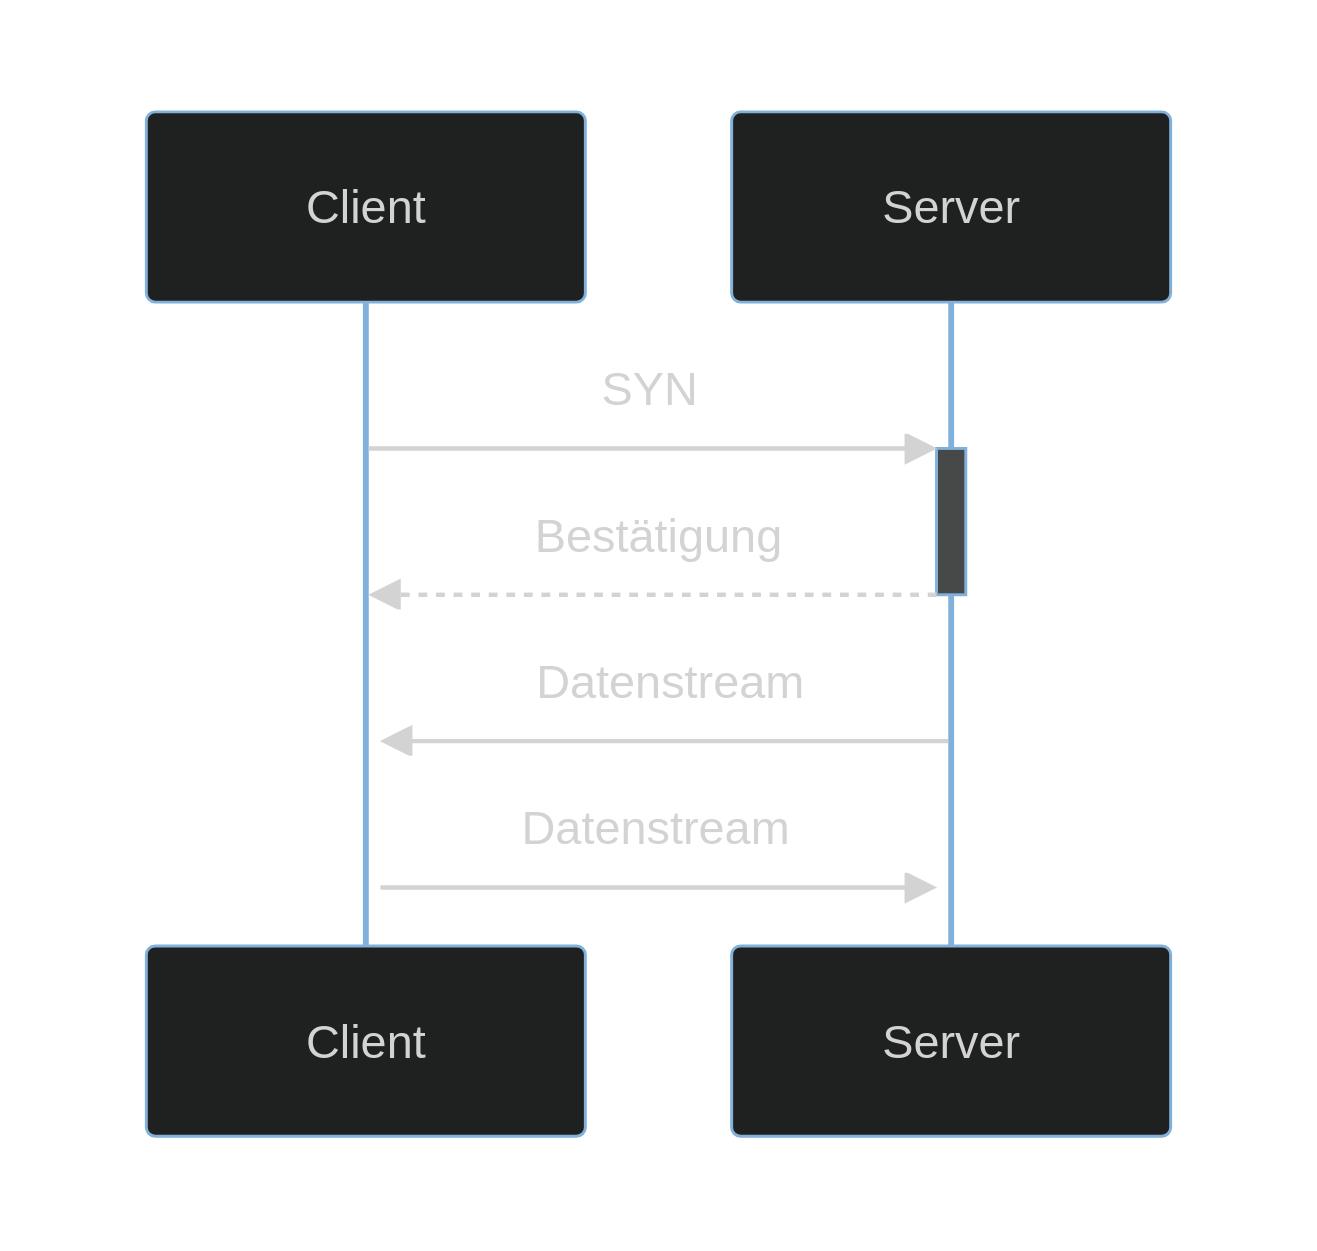
\includegraphics[scale=0.12]{Bilder/Datenfluss_TCP}
	\caption{Datenflussdiagramm für das Protokoll TCP\cite{datenflussdiagramm-tcp}}
	\label{fig:figure6}
\end{wrapfigure}
\vspace{-10pt}
Der Verbindungsaufbau läuft wie folgt ab: 
Der Client sendet eine Anfrage zum Verbindungsaufbau\footnote{SYN-Paket} zum Server. Wenn dies möglich ist, sendet der Server eine Bestätigung\footnote{ACK-Paket} zurück und baut den Kanal auf. Jetzt können der Client und Server miteinander kommunizieren und die Daten können übertragen werden. Wenn ein Datenpaket fehlerhaft übertragen wird, wird es nochmal geschickt.\cite{tcp-elektronik-kompendium} In Abbildung 5 ist dieser Datenverkehr in einem Datenflussdiagramm dargestellt. 
\newpage
UDP ist ein simpleres und verbindungsloses Protokoll. Das System für Fehlerkontrolle ist minimal, weswegen die korrekte Datenübertragung nicht garantiert ist. Die Daten werden kontinuierlich zum Empfänger geschickt, auch wenn dieser diese nicht empfängt. Dies macht UDP nicht ideal für das Verschicken von Dateien, aber um so besser zum streamen. Da das Protokoll wesentlich schneller ist, kann es mit einer höheren Bandbreite arbeiten, wenn diese nötig ist. Eine Fehlerkontrolle ist bei Streams aufgrund der Datenmenge nicht möglich. UDP ist somit Ideal für das Umsetzen von Videocalls, VoIP\footnote{Voice over IP} oder das Livestreamen auf Videoportalen oder im Fernsehen.\cite{udp} Die genauen Eigenschaften sind in Tabelle 3 dargestellt. 

\begin{table}[h]
	\resizebox{\textwidth}{!}{%
		\begin{tabular}{|
				>{\columncolor[HTML]{C0C0C0}}l |
				>{\columncolor[HTML]{eb5b34}}l |}
			\hline
			\cellcolor[HTML]{9B9B9B}Eigentschaften                        & \cellcolor[HTML]{9B9B9B}UDP                                                                       \\ \hline
			Verbindungsstatus                     & Verbindungslos, keine weiteren Anforderungen \\ \hline
			Datensequenzierung                    & Keine Sequenzierung                                                                               \\ \hline
			Garantierte Übertragung               & Keine garantierte Übertragung                                                                     \\ \hline
			Neuübertragung von verlorenen Paketen & Keine Neuübertragung von verlorenen Paketen                                                       \\ \hline
			Fehlerüberprüfung                     & Minimale Fehlerberprüfung durch Checksums                                                         \\ \hline
			Geschwindigkeit                       & Schneller als TCP                                                                                 \\ \hline
			bestmögliche Verwendung               & Schicken von Dateien, Email, Bilder, Websites, etc.                                               \\ \hline
		\end{tabular}%
	}
	\caption{UDP \cite{udp+tcp}}
	\label{fig:figure10}
\end{table}
	
\begin{wrapfigure}{r}{0.5\textwidth}
	\centering
	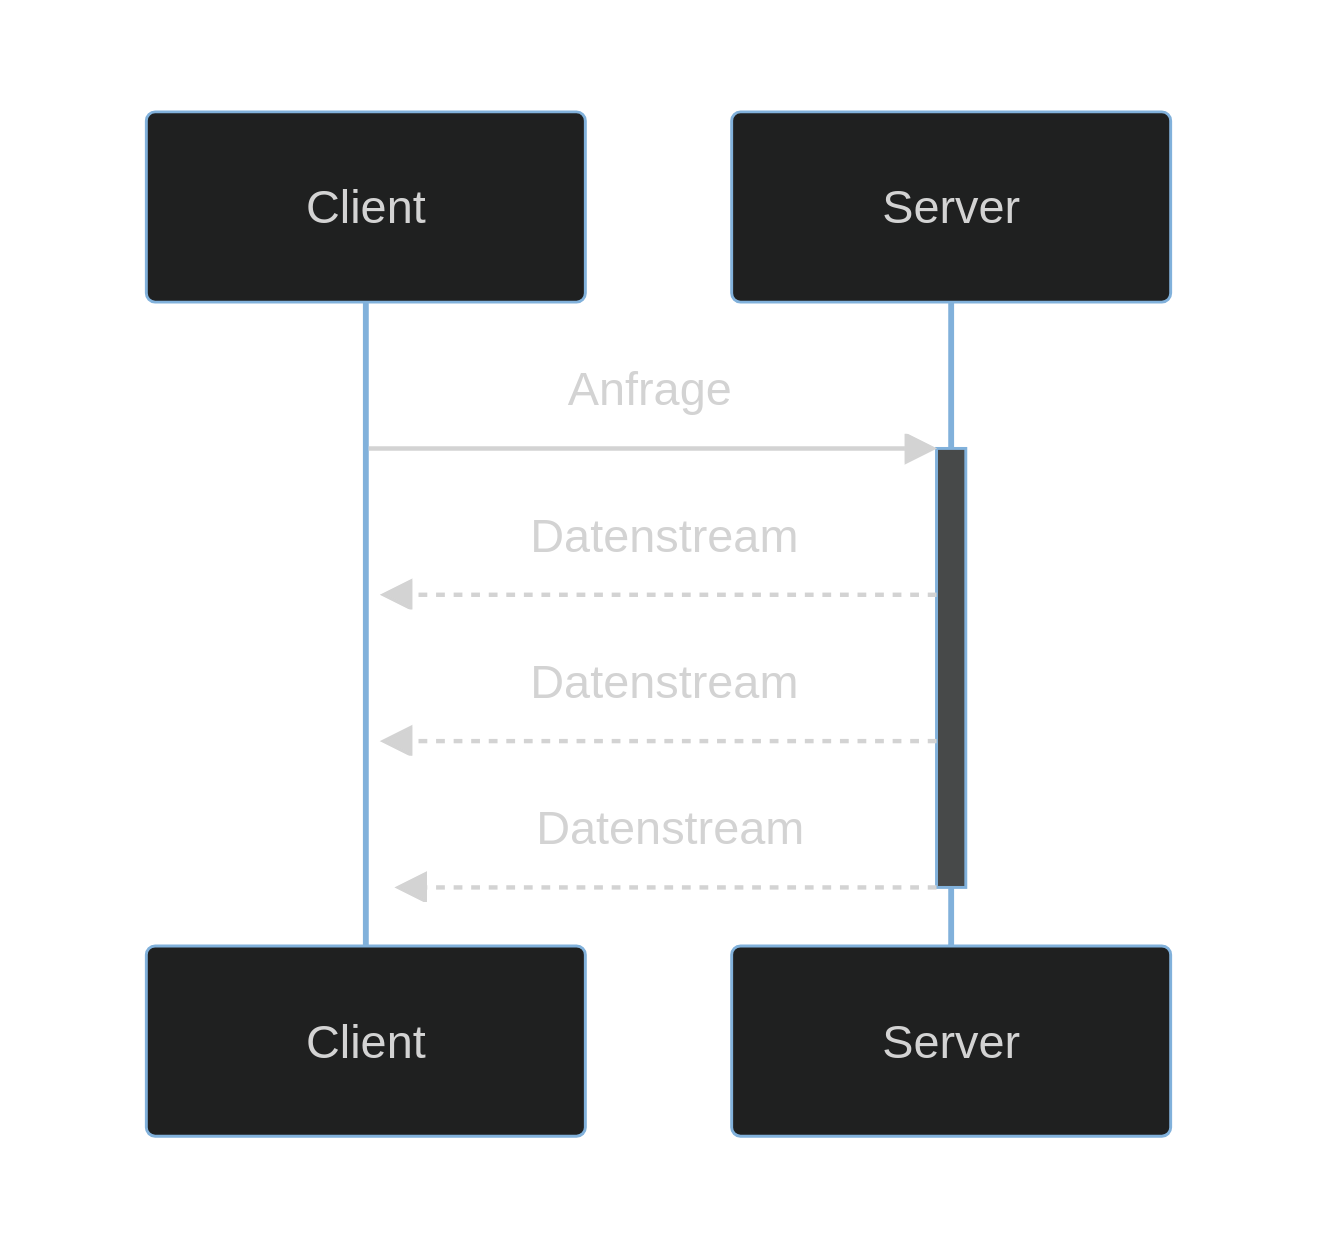
\includegraphics[scale=0.12]{Bilder/Datenfluss_UDP}
	\caption{Datenflussdiagramm für das Protokoll UDP\cite{datenflussdiagramm-udp}}
	\label{fig:figure7}
\end{wrapfigure}

Der Verbindungsaufbau läuft wie folgt ab: Der Client schickt dem Server ein Anfrage, in welcher die Öffnen des Streams erbittet wird. Daraufhin antwortet der Server direkt mit dem Datenstream. Dieser Stream bleibt geöffnet, auch wenn der Client den Datenstream nicht mehr aufnimmt. Der Server muss den Transfer eigenständig stoppen, wenn Bandbreite gespart werden muss.
In Abbildung 6 ist der Datenverkehr in einem Datenflussdiagramm dargestellt.\cite{udp-elektronik-kompendium}

\subsubsection{Netzwerkschicht}
	Auf die Transportschicht folgt die Netzwerkschicht\footnote{engl: network layer}. Diese gewährt das Kommunizieren zwischen Geräten in verschiedenen, miteinander verbundenen Netzwerken. Beim Versenden werden die Segmente der Transportschicht erneut in kleinere Datenpakete aufgeteilt und mit weiteren Informationen versehen. Diese Informationen sind für die auf dem Weg gelegenen Knoten gedacht, um diesen das Ziel des Pakets aufzuweisen. Es wird der beste physikalisch mögliche Weg ausgesucht, um die Daten sicher an ihr Ziel zu bringen. Dieser Prozess wird Routing genannt.\cite{routing}
	Wenn sich beide Geräte im selben Netzwerk befinden, wird diese Ebene übersprungen. 
	
	Zu den Protokollen für diese Schicht gehören das IP\footnote{Internet Protocol}, das ICMP\footnote{Internet Control Message Protocol}, das IGMP\footnote{Internet Group Message Protocol} und die IPsec\footnote{Internet Protocol Security}. Ein Beispielgerät, welches in dieser Schicht agiert, wäre ein Router.\cite{osi-schichten-cloudflare}\cite{osi-schichten-netzwerkecom}
	
\subsubsection{Sicherungsschicht}
	Die Sicherungsschicht\footnote{engl: Data Link Layer} stellt die vorletzte Schicht dar. Diese ist der Netzwerkschicht sehr ähnlich. Der wesentliche Unterschied ist, dass die Sicherungsschicht für die Kommunikation von zwei Geräten innerhalb eines Netzwerks zuständig ist. Die Sicherungsschicht ist ebenfalls für die Fluss- und Fehlerkontrolle in der netzinternen Kommunikation zuständig. 
	
	Beispielgeräte für diese Ebene sind Bridges und Switches.\cite{osi-schichten-cloudflare}\cite{osi-schichten-netzwerkecom}

\subsubsection{Bitübertragungsschicht}
	Die unterste Schicht wird durch die Bitübertragungsschicht\footnote{engl: physical layer} dargestellt. Hier sind die Daten als Bitstrom vorhanden, eine Zeichenkette bestehend aus Einsen und Nullen. Hier muss sich auf mehrere Eigenschaften geeinigt werden. Zu Beginn müssen die Gegebenheiten des Übertragungsmediums festgelegt werden. Dies betrifft die Wahl des Materials und die Funktion der einzelnen Leitungen. Ein Kabel kann beispielsweise aus Kupfer oder Glasfaser bestehen und zwei innere Leitungen haben: eine Datenleitung und eine Steuerleitung. Bei der Übertragung über Funk wird beispielsweise durch Luft übertragen. Es muss ebenfalls die Übertragungsrichtung und Geschwindigkeit festgelegt werden. Ein Kabel kann in eine Richtung\footnote{simplex}, abwechselnd in beide Richtungen\footnote{halb-duplex} oder in beide Richtungen gleichzeitig\footnote{duplex} übertragen.\cite{osi-schichten-cloudflare}\cite{osi-schichten-netzwerkecom}


\section{Analyse}
In der Analyse soll häufig benutzte Software getestet werden. Ich habe mich für einen Webbrowser entschieden, da diese am meisten benutzt werden.\cite{beliebteste-programme} Zu Beginn soll die Wireshark-Installation getestet werden. Hierfür habe ich einen simplen Test erstellt.

\subsection{Beispiel}
In diesem Kapitel wird eine Beispielkommunikation vereinfacht dargestellt werden. Es wird ein lokaler Webserver erstellt und anschließend kontaktiert. Dieser Transfer wird dann durch Wireshark aufgezeichnet.

\subsubsection{Webserver}
Code: 

\begin{lstlisting}
	from flask import Flask #importieren von den benoetigten Bibliotheken
	import os
	from datetime import datetime
	
	hostName = "localhost" #setzen des Hostnamen
	serverPort = 8080 #setzen des Ports (Erklaerung unter dem Code)
	app = Flask(__name__) #der Flask Server wird instanziert
	@app.route('/') #wenn zum index geroutet wird...
	def index():
	return '<p>willkommen in der http webserver demo</p>'  #...soll diese response zurueckgeschickt werden
	@app.route('/time') #wenn zu /time geroutet wird...
	def time():
	now = datetime.now()
	current_time = now.strftime("%H:%M:%S") #erstellen der response
	return f'Jetzige Zeit: {current_time}' #...soll diese response zurueckgeschickt werden
	
	if __name__ == '__main__':
	app.run(host=hostName, port=serverPort) #starten des Servers
\end{lstlisting}

Mit der `flask` Bibliothek können Webserver in der Programmiersprache Python leicht umgesetzt werden. Sie erlaubt es Webserver zu erstellen, die auf Anfragen hören und mit dem angefragten Inhalt antworten können.\cite{flask}

\paragraph{Weitere Erklärung zum Code:}
\glqq Ports sind ein Merkmal der Protokolle TCP und UDP\grqq\cite{ports19}. Diese werden benutzt, um den Datenverkehr zu ordnen. Da auf einem Server oft mehrere Programme aktiv sind, die gleichzeitig über das Netzwerk kommunizieren, müssen diese eingeteilt werden, sodass die Pakete nicht durcheinander kommen. Jedes Programm legt seinen Port fest bzw. bekommt vom Betriebssystem einen Port zugewiesen. Dieser kann zwischen 0 und 65535 liegen.\cite{ports}

Anschließend wird Wireshark geöffnet und das richtige Netzwerkinterface, welches aufgenommen werden soll, ausgewählt. In `diesem Fall ist es das \glq Loopback:io\grq interface. (siehe: Anlagen, Das Wireshark interface, auswählen des Loopback Geräts)
\subsubsection{Loopback Interface}

Das \glq Loopback Interface\grq ist eine \glqq Pseudo-Netzwerkschnittstelle zum gefahrenlosen Testen\grqq\cite{loopback-munich}. Der Netzwerkverkehr wird in diesem Fall im genannten Netzwerkinterface zu sehen sein, da der Server auf \glq localhost\grq live ist. Das \glq Loopback Interface\grq agiert als virtuelle Netzwerkkarte und ist nicht wirklich als Hardware vorhanden. Da ich diesen Test auf einem Linux Betriebssystem durchführe, wird diese Funktion durch Wireshark unterstützt.\cite{loopback-wireshark}

\subsubsection{Ergebnis}

Nun muss der Server kontaktiert werden. Dies kann man mit einem Webbrowser machen. Mit Firefox habe ich dann \glq http://localhost:8080\grq kontaktiert. In Wireshark sind direkt mehrere neue Einträge zu erkennen. (siehe: Anlagen, der Datentransfer wurde aufgezeichnet)

Im nächsten Schritt wird die erste Anfrage, mit dem \glq HTTP\grq Protokoll angesehen. (siehe: Anlagen, Analyse des \glq GET\grq requests). Unten rechts ist der Inhalt des Pakets zu erkennen. Darin sind einige Daten zum Browser enthalten und zum Inhalt, welcher angefragt wird. Diese Daten werden später in der Analyse weiter durchleuchtet.

Der Server antwortet mit diesem angeforderten Inhalt (siehe: Anlagen, Analyse der response). Der Inhalt ist, der oben im Code festgelegte Satz, ``Willkommen in der http Webserver demo``

\subsection{Browser}

In dieser Analyse wird hauptsächlich auf das DNS\footnote{Domain Name System} Protokoll geschaut. Dieses Protokoll erlaubt dem Client mit dem \glq Domain Name System\grq zu kommunizieren. Dieses System besteht aus Servern, die Hostnamen in IP-Adressen umwandeln können. Hostnames sind die von Menschen erkennbaren Adressen von Websites, wie \glq google.com\grq oder \glq luisherzog.de\grq. IP-Adressen sind die von Rechnern verstehbaren Adressen von Servern, wie z.B. \glq 192.169.11.4\grq oder \glq 115.234.34.2\grq. Das DNS-System enthält eine Liste dieser Hostnames mit den dazugehörigen IP-Adressen. Wenn wir beispielsweise mit dem Browser eine Website besuchen wollen, wird durch das DNS-Protokoll eine Anfrage an das DNS-System mit der URL\footnote{Uniform Resource Locator} geschickt. In der URL ist der Hostname des Servers enthalten. Das DNS-System sucht in der Liste und leitet das Datenpaket auf den Weg zum Zielserver.\cite{dns-cloudflare} Im Netzwerk wird diese Aufgabe durch den Router übernommen.

Durch das Analysieren des DNS-Verkehrs, kann man herausfinden, welche Server kontaktiert werden. Der Dateninhalt des Pakets ist oft verschlüsselt und somit unlesbar, was eine tiefere Analyse der verschickten Daten unmöglich macht. 

Ich habe mich beispielsweise mit dem Firefox Browser auseinandergesetzt. Die meisten Browser agieren im Netzwerkverkehr ähnlich.

\subsubsection{Firefox}

Beim Öffnen  von Firefox werden mehrere Anfragen an das DNS-System getätigt. 
\begin{enumerate}
	\item Firefox macht die IP-Adresse des Routers im Heimnetzwerk ausfindig. 
	\item Firefox schaut, ob ein Captive Portal vorhanden ist. \glqq Ein Captive Portal ist eine Webseite, die der Benutzer eines öffentlich zugänglichen Netzwerks ansehen und mit ihr interagieren muss, bevor der Zugang gewährt wird.\grqq\cite{captiveportal-computerweekly} Diese sind oft in öffentlichen Plätzen, wie Flughäfen, Cafés oder in Schulnetzwerken verwendet. Dies erzielt Firefox mit dem Kontaktieren der Adresse \glq detectportal.firefox.com\grq. Hierbei testet Firefox ebenfalls, ob das Netzwerk andere Technologien,  wie IPv6 unterstützt.\cite{captiveportal-firefox}
	\item Die Adresse \glq api.accounts.firefox.com\grq wird von Firefox kontaktiert. Dies liegt höchstwahrscheinlich daran, dass ich einen Firefox Account benutze und dadurch automatisch angemeldet werde.
	\item Diese Anfrage ist kontroverser zu betrachten. Die Anfrage geht an \glq incoming.telemetry.mozilla.org\grq. Was hier genau verschickt wird, ist unbekannt. Der Adresse nach zu urteilen, handelt es sich hier um Messungsdaten, die Firefox aufnimmt und an die Entwickler schickt, um Firefox zu verbessern. Welche Daten das genau sind und ob diese Daten ggf. die Privatsphäre der Nutzer beeinträchtigen, kann aus Wireshark nicht ausgelesen werden, da der Inhalt verschlüsselt ist.
	\item Firefox kontaktiert die Adresse \glq push.services.mozilla.com \grq. Hier wird der Adresse nach zu urteilen, nach Push-Benachrichtigungen gesucht, die noch zugestellt werden müssen. 
	\item \glq token.services.mozilla.com\grq ist die nächste Adresse, die kontaktiert wird. Hierbei geht es um die Sync Funktionalität eines Firefox Accounts. Firefox schaut hier, ob sich der synchronisierte Inhalt innerhalb eines Firefox Accounts verändert hat. Dies betrifft beispielsweise Tabs, Lesezeichen und zuletzt besuchte Websites. Diese Anfrage ist gut dokumentiert und erlaubt es somit, diese Funktion auch selbst zu hosten.\cite{syncstorage-firefox} Bei mir wurde es unter \glq prod.tokenserver.prod.cloudops.mozgcp.net\grq gehostet, was die nächste Adresse war, die kontaktiert wurde.
	\item Zuletzt wird den Extensions erlaubt, Anfragen zu stellen. Davor wird noch die Adresse \glq services.addons.mozilla.org \grq kontaktiert, wahrscheinlich um nach updates für die jeweiligen Extensions zu schauen.
\end{enumerate}
\newpage
	Hierbei muss beachtet werden, dass Firefox noch viel mehr Anfragen stellt. Diese gehen zumeist an Zertifikatstationen, um die Sicherheit der Verbindung zu gewähren. Ebenso werden Adressen auch mehrfach kontaktiert, was in der oberen Liste nicht mit inbegriffen ist. Die Abbildung 7 zeigt den Umfang der Anfragen.
	
\begin{figure}[h]
	\centering
	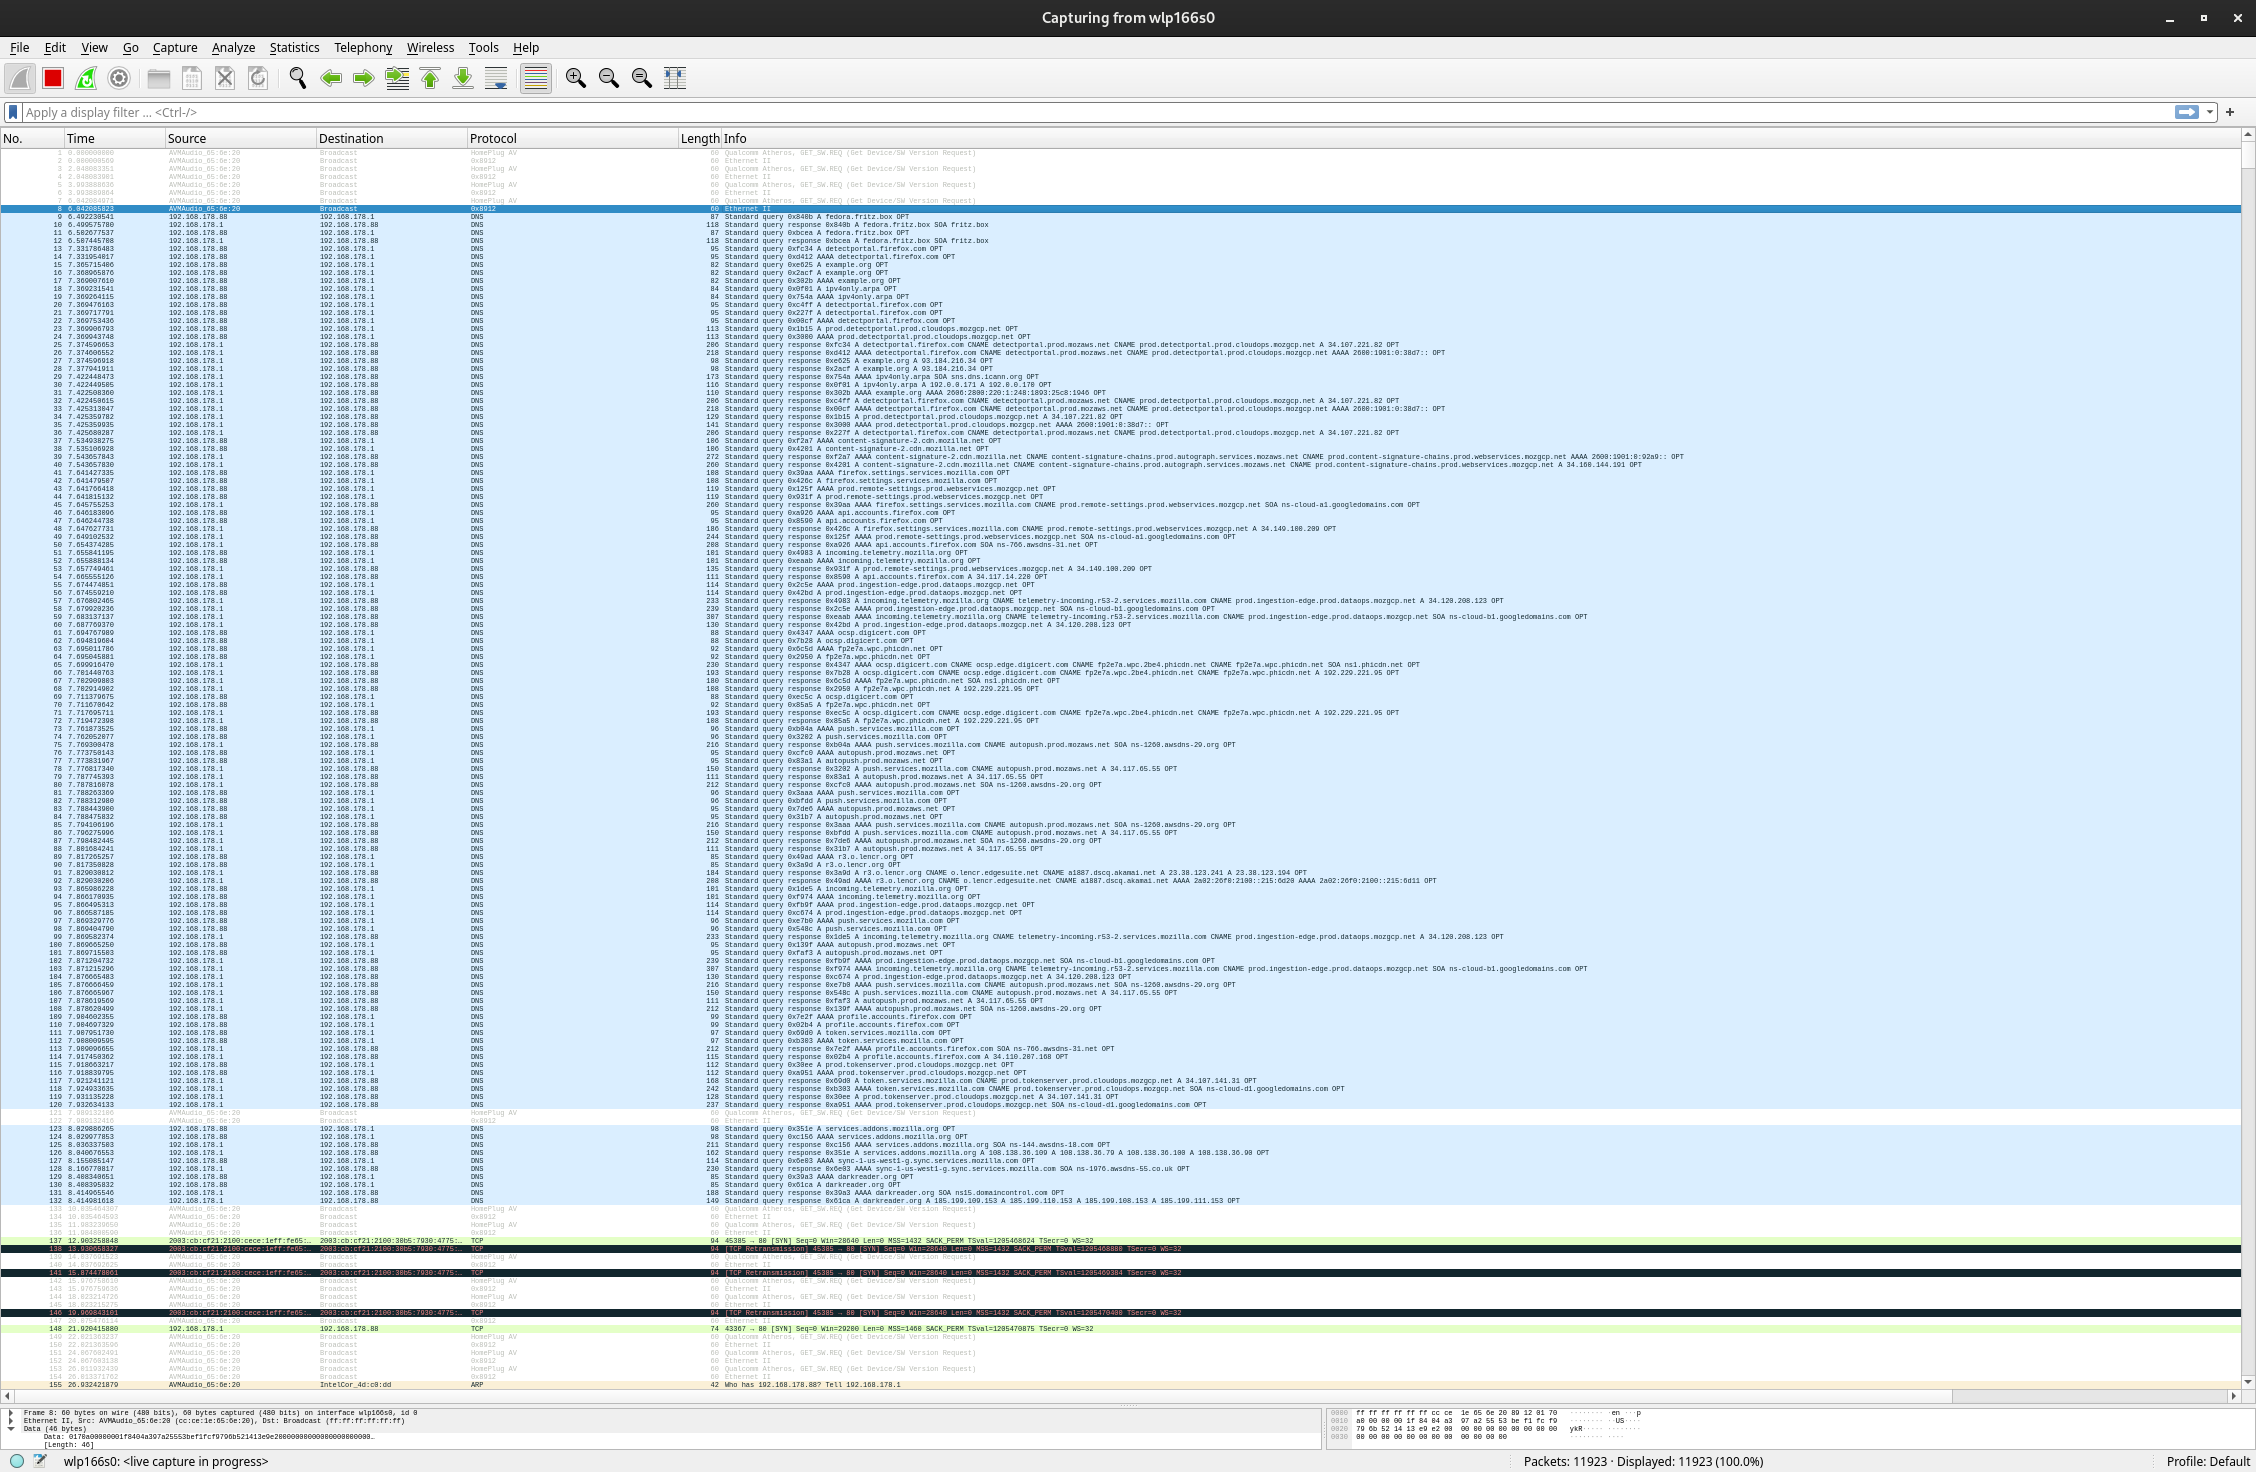
\includegraphics[scale=0.18]{Bilder/firefox-anfragen}
	\caption{Firefox tätigt sehr viele Anfragen\cite{screenshots-self}}
	\label{fig:figure12}
\end{figure}

\section{Fazit}

Dieses Thema hat mir sehr viel gezeigt. Mir war vorher nicht klar, wie viel wirklich im Netzwerk vor sich geht. Sobald man die Wireshark Software öffnet, wird man direkt mit mehreren Anfragen überschwemmt. Ich finde es trotzdem bemerkenswert, wie der Datenverkehr durch die ganzen oben genannten Schritte optimiert und effizienter gestaltet wird. Jedes einzelne Konzept ist sehr durchdacht und für einen bestimmten Zweck optimiert. Ich finde es trotz dessen schwierig auf Frage \glqq Was passiert im Netzwerk?\grqq zu antworten. Wie in dieser Arbeit festgestellt gibt es viele verschiedene Arten von Netzwerken mit verschiedenen Verwendungszwecken. Jedes Netzwerk bietet somit unterschiedliche Voraussetzungen, die zu verschiedenen Ergebnissen führen. Die Frage, was wirklich übertragen wird, spielt in diesem Sinne ebenfalls eine große Rolle. Bevor ich zu diesem Thema recherchiert habe, war ich den Metadaten in Protokollheadern negativ gegenüber gestanden. Ich habe diese immer als Tracker, zum Sammeln von personenbezogenen Daten angesehen. Jetzt weiß ich mehr. Mir ist klar geworden, dass der Datenverkehr ohne diese Metadaten nicht funktioniert. Spongebob aus der Kinderserie \glqq Spongebob Schwammkopf\grqq wollte das Wasser vorher auch nicht bekommen. Zum Schluss fällt allerdings auf, dass er ohne Wasser ebenso wenig funktioniert, wie der Datenverkehr ohne Metadaten.


\begin{figure}[h]
	\centering
	
\includegraphics[scale=0.5]{Bilder/Spongebob}
	\caption{Spongebob funktioniert nicht ohne Wasser\cite{spongebob}}
	\label{fig:figure99}
\end{figure}


% end of text






\newpage
 \listoffigures
 \listoftables
\newpage
\bibliographystyle{plain}
\bibliography{gg}

\newpage
\fancyhead{}
\renewcommand{\headrulewidth}{0pt}
\vspace*{40pt}
\begin{center}
	\large{Ich erkläre hiermit, dass ich die Seminararbeit ohne fremde Hilfe angefertigt und nur die im Literaturverzeichnis angeführten Quellen und Hilfsmittel benützt habe.}
	\vspace{40pt}
	\hrule
\end{center}
	\scriptsize{\textit{Ort, Datum, Unterschrift des Verfassers}}

\newpage
\pagestyle{empty}
\centering
\vspace*{200pt}
\Huge{\section{Anlagen}}
\newpage

\begin{figure}[h]
	\centering
	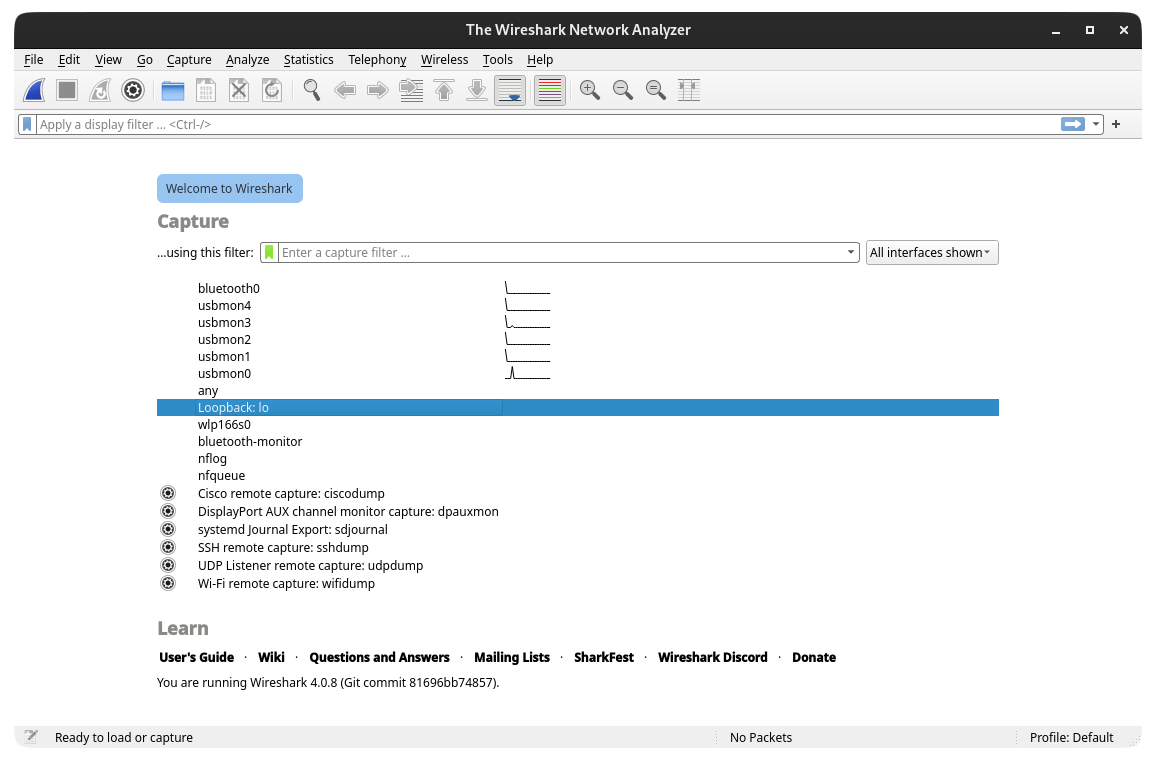
\includegraphics[scale=0.3]{Bilder/Anlagen_1}
	\caption{Das Wireshark interface, auswählen des Loopback Geräts \cite{screenshots-self}}
	\label{fig:figure30}
\end{figure}

\begin{figure}[h]
	\centering
	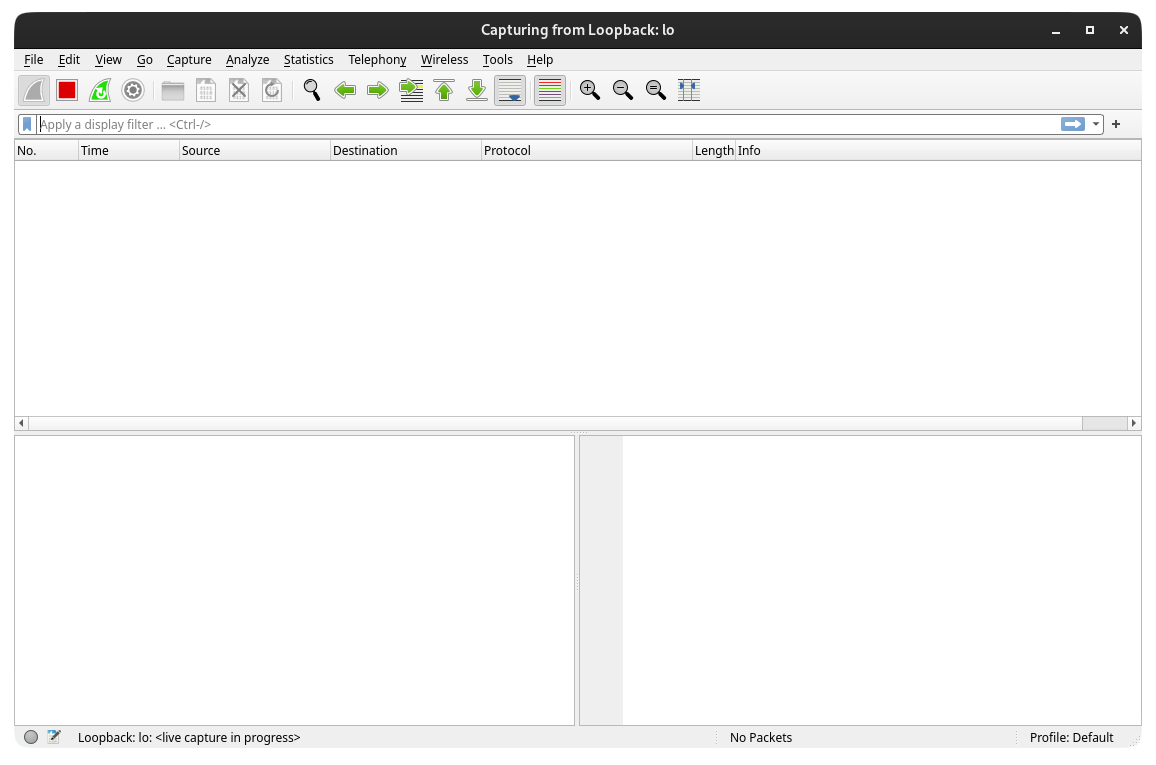
\includegraphics[scale=0.3]{Bilder/Anlagen_2}
	\caption{Das Wireshark interface, warten auf Datentransfer \cite{screenshots-self}}
	\label{fig:figure31}
\end{figure}

\begin{figure}[h]
	\centering
	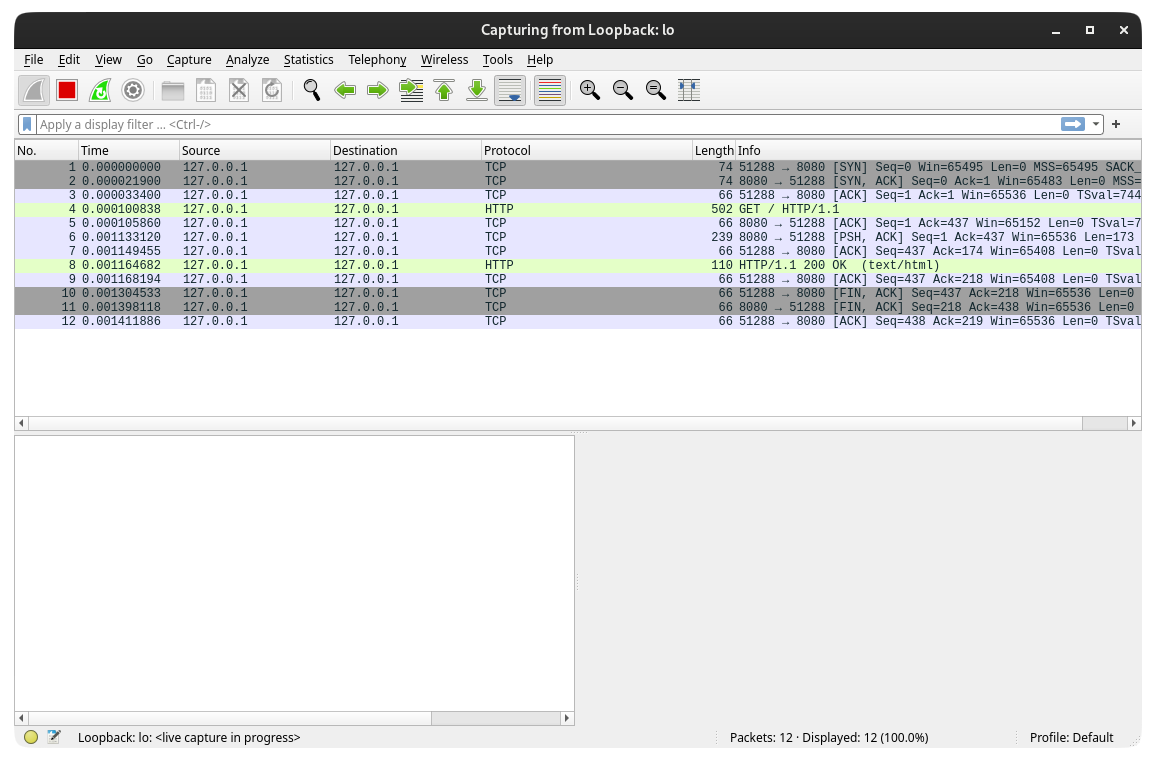
\includegraphics[scale=0.3]{Bilder/Anlagen_3}
	\caption{Das Wireshark interface, der Datentransfer wurde aufgezeichnet\cite{screenshots-self}}
	\label{fig:figure32}
\end{figure}

\begin{figure}[h]
	\centering
	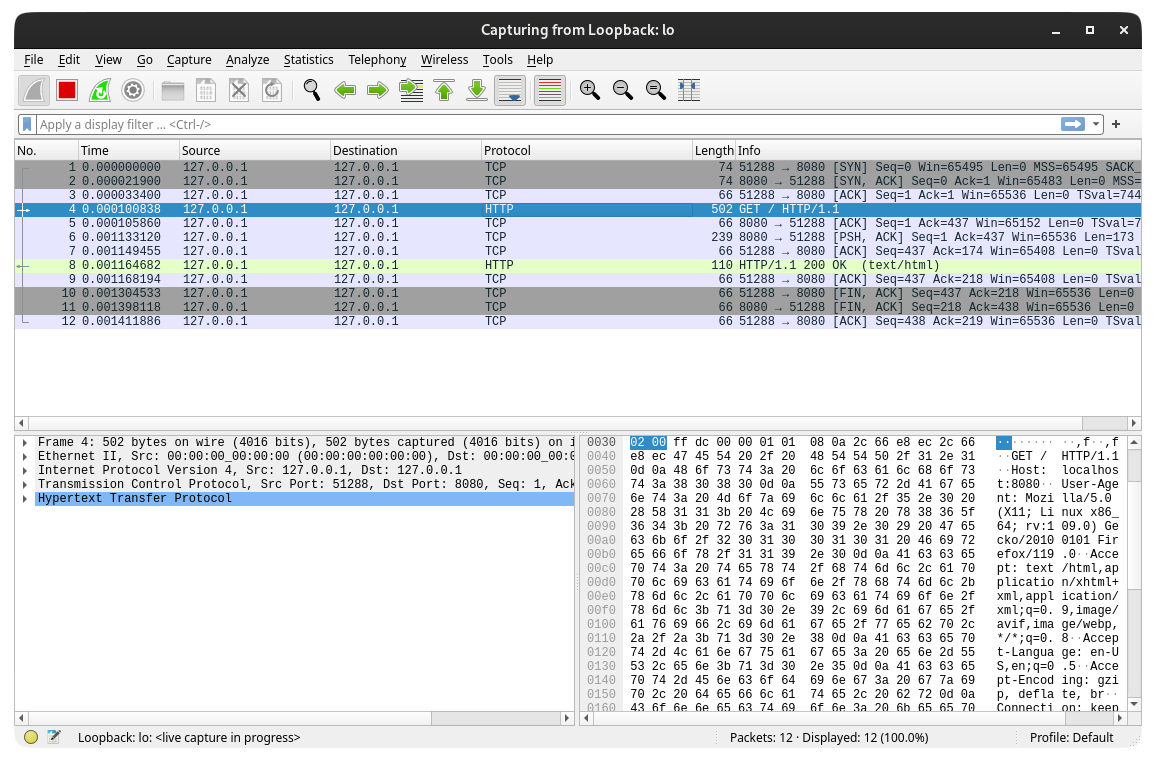
\includegraphics[scale=0.3]{Bilder/Anlagen_4}
	\caption{Das Wireshark interface, Analyse des `GET` requests \cite{screenshots-self}}
	\label{fig:figure33}
\end{figure}

\begin{figure}[h]
	\centering
	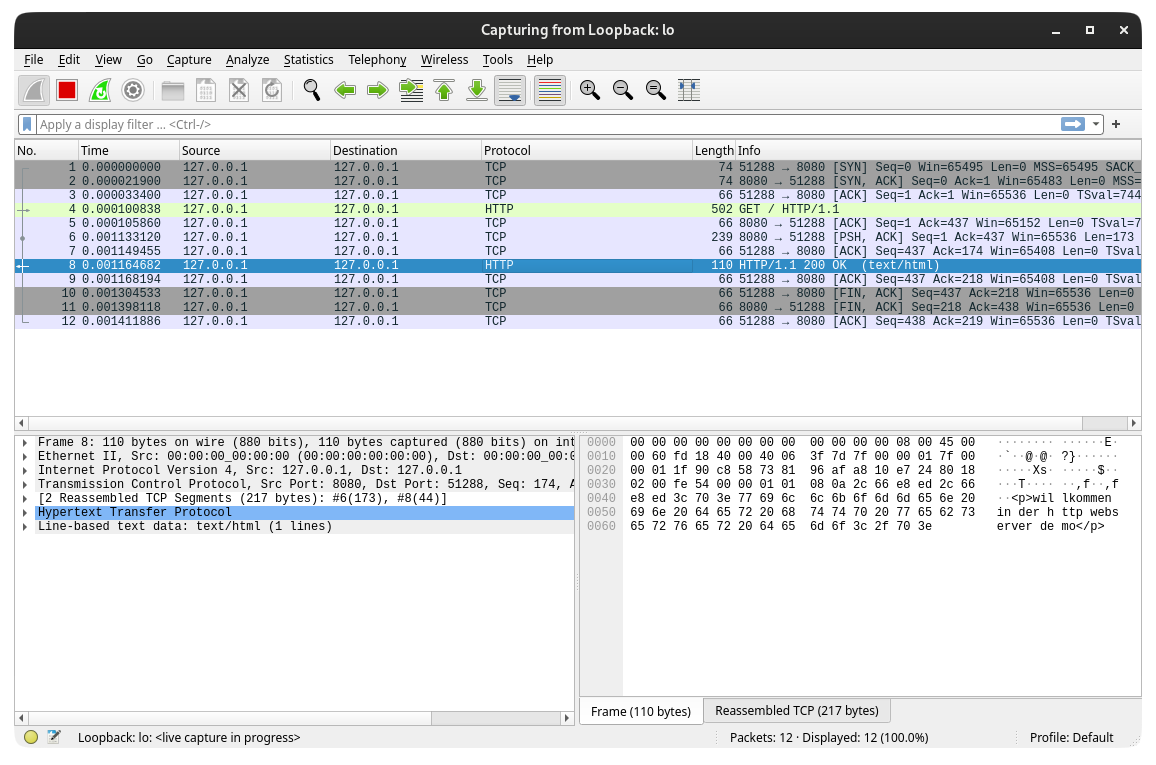
\includegraphics[scale=0.3]{Bilder/Anlagen_5}
	\caption{Das Wireshark interface, Analyse der response \cite{screenshots-self}}
	\label{fig:figure34}
\end{figure}


\end{document}

